 
   %judul bisa diketik ulang
  \setstretch{1}%\small
  \begin{center}
      \textbf{\large \Title}\\
      \bigskip 
  \end{center}
  
  
  
  %Nama authors
   \begin{center}
     \bf \Author$^1$, Mira Kania Sabariah$^2$, Monterico Adrian$^3$
  \end{center}
  
  
  %Afiliasi dan email
   \begin{center}
     $^{1,2,3}$Fakultas Informatika, Universitas Telkom, Bandung\\
$^4$Divisi Digital Service PT Telekomunikasi Indonesia\\
$^1$rovino@students.telkomuniversity.ac.id, $^2$mirakarnia@telkomuniversity.ac.id,\\ $^3$monterico@telkomuniversity.ac.id
  \end{center}
  
   
 %%% Abstrak Indonesia %%%%%%%%%%  
   
{\bf \parindent0pt \noindent\rule{\textwidth}{1pt}
Abstrak

Populasi penduduk yang tinggi di Indonesia mengakibatkan antrian panjang dalam berbagai pelayanan publik atau pelayanan konsumen. Pelanggan harus datang ke tempat untuk mengambil antrian dan menunggu gilirannya, semakin panjang antrian, semakin lama waktu tunggu yang dibutuhkan. Hal ini tidak efisien dan menyebabkan banyak waktu terbuang hanya untuk menunggu antrian. Jika nomor antrian bisa didapatkan secara online dan dapat dipantau secara online, maka dapat mengurangi waktu yang terbuang. Dengan aplikasi antrian virtual dapat memperpendek antrian secara fisik, dengan cara antri secara virtual, melihat antrian yang sedang berjalan, dan booking tempat. Pada Pengembangan aplikasi ini, framework yang digunakan adalah NestJS dan PrismaJS dengan menerapkan RESTful API, Object Relational Mapping, dan menghindari Anti-Pattern. Framework NestJS mendukung pembuatan aplikasi ber-arsitektur monolitik dan \textit{microservice}. Setelah aplikasi dibangun di arsitektur monolitik, aplikasi dapat dengan mudah dimigrasikan ke \textit{microservice} saat penggunaan aplikasi sudah hampir mendekati batas muat pengguna.\\

 \bigskip
Kata kunci : NestJS, PrismaJS, Anti-Pattern, Antrian, Backend, REST



%%% Abstrak English %%%%%%%%%%  



\noindent\rule{\textwidth}{1pt}
Abstract

The abstract should state briefly the general aspects of the subject and the main concolusions.  The length of abstract should bo no more than 200 word and  should be typed be with 10 pts.

 \bigskip
Keywords: keyword should be chosen that they best describe the contents of the paper and should be typed in lower-case, except abbreviation. Keyword should be no more than 6 word 

\noindent\rule{\textwidth}{1pt} }
   


%%%%%% isi paper %%%%

\section{Pendahuluan}

\noindent\textbf{Latar Belakang}

Meningkatnya populasi di indonesia mengakibatkan banyak pelanggan ya-ng mengantri untuk mendapatkan layanan di bank, restoran, rumah sakit, dan tempat penyedia jasa lainnya. Mengantri merupakan kegiatan yang membosankan dan menguras waktu. Panjangnya antrian juga mampu berdampak pada mutu pelayanan di suatu tempat. Pelanggan yang harus menunggu lama berpotensi beralih ke pesaing, atau jika ada urusan lain yang lebih penting, maka pelanggan akan keluar dari tempat antrian, meninggalkan antriannya \cite{khong2017queue}\cite{Ghazal2016}\cite{Uddin2016}. Solusi yang ada pada bank, kantor pos, dan rumah sakit saat ini menggunakan \textit{ticketting} nomor antrian secara manual, dimana antrian yang sedang dilayani ditampilkan di layar pada ruang tunggu. Hal ini kurang efektif karena pelanggan harus berada di ruang tunggu\cite{Ghazal2016}.

Perkembangan teknologi yang cepat mengakibatkan penggunaan perangkat pintar atau \textit{smartphone} merupakan hal lumrah, banyak bermunculan aplikasi antrian virtual seperti Antrique, Qiwee, ExaQue dimana pengguna dapat mengantri dari jarak jauh melalui aplikasi maupun \textit{website}. Para pengguna aplikasi tersebut dapat melakukan hal lain saat mengantri sebelum gilirannya. Namun, aplikasi-aplikasi tersebut memiliki banyak kelemahan seperti \textit{UI/UX} yang tidak bagus, sering \textit{crash} dan \textit{freeze}, tidak ada estimasi waktu antrian, dan masih belum ada yang berfokus ke sektor \textit{food and beverage}.

Oleh karena itu, perlunya dikembangkan sebuah aplikasi yang memiliki fitur yang sama atau lebih dengan menutup kekurangan pada aplikasi tersebut. Pengembangan aplikasi yang direncanakan menggunakan arsitektur monolitik karena mudahnya untuk dibuat dan di-\textit{deploy} secara cepat untuk di iterasikan. Namun, arsitektur monolitik memiliki kelemahan seperti sulitnya untuk di-\textit{maintenance}, \textit{scale}, dan reliabilitas nya. Oleh karena itu, perlu diperhatikan bagaimana cakupan aplikasi kedepannya dan perlunya migrasi ke arsitektur \textit{microservice} \cite{gos2020comparison} \cite{jatkiewicz2023differences}.

Dalam pengembangan aplikasi web, pemilihan bahasa pemrograman untuk digunakan di \textit{backend} sangatlah penting karena dapat mempengaruhi performa aplikasi yang dibangun. Dalam pemilihan bahasa pemrograman \textit{backend}, banyak pilihan yang tersedia seperti PHP, Python, Ruby, PERL, dan banyak lagi. NodeJs merupakan \textit{tools} yang memungkinkan bahasa JavaScript dapat dijalankan pada sisi \textit{backend}. Dalam sisi performa, NodeJs lebih unggul dibanding PHP dan Python dalam sisi kecepatan melayani \textit{request} dari client \cite{William2020} \cite{Odeniran2023}.

NestJs merupakan \textit{framework backend} dari Nodejs yang menggunakan bahasa typescript, dan bisa digunakan untuk pengembangan arsitektur berbasis \textit{microservice} dan monolitik, jadi jika aplikasi dikembangkan pada arsitektur monolitik dapat dengan mudah dimigrasikan ke \textit{microservice}. NestJs juga bisa digunakan bersamaan dengan \textit{framework} PrismaJs untuk mengelola database \cite{NestJS}. PrismaJs merupakan \textit{framework} Object Relational Mapping (ORM) \cite{Prisma}, digunakan untuk mempercepat, dan mempermudah pengembangan aplikasi yang database-nya memiliki relasi yang kompleks dan sulit di-\textit{maintenance} jika menggunakan Structured Query Language (SQL) \cite{Zmaranda2020}.

Implementasi Application Programming Interface (API) yang digunakan adalah Representational State Transfer (RESTful) API, RESTful API adalah arsitektur untuk mempermudah komunikasi client-server agar efektif untuk transaksi data. Namun, pada implementasi RESTful API, ada beberapa hal yang perlu diperhatikan seperti keamanan saat transaksi  atau komunikasi \cite{Beer2018}. Keamanan yang lemah dapat mengakibatkan hacker dapat dengan mudah melakukan \textit{request tampering}, mengambil data pengguna, dan dapat membocorkan data keuangan mitra. \textit{Design pattern} juga perlu diperhatikan dalam penggunaan bahasa untuk API \textit{endpoint} nya agar tidak terjadi \textit{anti pattern}. \textit{Anti pattern} terjadi saat penamaan API tidak sesuai dengan fungsi, atau ada fungsi sejenis tapi penamaannya berbeda jauh. Dengan menghindari \textit{anti pattern}, dapat berakibat ke aplikasi yang lebih mudah di-\textit{sustain} dan di-\textit{maintain} \cite{Aghajani2018} \cite{Alshraiedeh2021}.

Berdasarkan uraian di atas, penelitian ini akan membuat sebuah \textit{backend} aplikasi antrian dengan menggunakan arsitektur monolitik dengan \textit{framework} NestJs dan PrismaJs sebagai \textit{framework} nya. Setelah fitur-fitur aplikasi dibuat, perlu dilakukan unit testing untuk memvalidasi kodingan yang telah ditulis. Hal ini bertujuan untuk meminimalisir bug dan mencegah terjadinya regresi saat fitur baru ditambahkan \cite{runeson2006survey}.\\

\noindent\textbf{Topik dan Batasannya}

Aplikasi antria memerlukan backend developer untuk mengimplementasi-kan fungsi fungsi API dan manajemen database nya. Maka dapat dirumuskan permasalahan sebagai berikut:
\begin{enumerate}
  \item Bagaimana meningkatkan \textit{maintainability} penggunaan database pada projek.
  \item Bagaimana merancang API yang bebas dari \textit{anti pattern}.
  \item Bagaimana merancang sistem keamanan pada API untuk melayani \textit{request}.
\end{enumerate}
dan batasan masalah sebagai berikut:
\begin{enumerate}
  \item Hanya berfokus kepada implementasi database menggunakan Prisma ORM.
  \item Berfokus ke bagaimana membuat \textit{endpoint} API yang tidak menimbulkan \textit{anti pattern}.
  \item Implementasi keamanan pada saat penanganan \textit{request} menggunakan JSON Web Token (JWT).
\end{enumerate}


\noindent\textbf{Tujuan}

Tujuan dari pengerjaan Tugas Akhir ini yaitu:
\begin{enumerate}
  \item Mengimplementasikan Prisma ORM untuk meningkatkan \textit{maintainability} pada penggunaan database.
  \item Membuat dokumentasi API yang dapat dengan mudah dimengerti dan di \textit{maintain}.
  \item Mengamankan data pengguna dengan memerlukan \textit{Authorization} pada setiap header request.
  
\end{enumerate}

% \noindent \textbf{Organisasi Tulisan}

% Pada sub-bagian ini dituliskan bagian-bagian selanjutnya (setelah Pendahuluan) pada jurnal TA ini, disertai penjelasan sangat singkat.

\section{Kajian Pustaka}
\subsection{NodeJs}
NodeJs adalah \textit{runtime} javascript yang basisnya dibangun dari V8 Java-Script Engine. NodeJs berjalan dalam bentuk \textit{event-driven}, dan menggunakan model \textit{non blocking I/O}. meskipun menggunakan \textit{event-driven} untuk melayani \textit{request}, NodeJs dapat melayani jutaan koneksi dalam waktu bersamaan secara \textit{asynchronous} \cite{shah2017node}.

\subsection{NestJs}
NestJs merupakan \textit{framework} untuk Nodejs yang dikembangkan oleh Kamil Myśliwiec yang bertujuan untuk membuat aplikasi NodeJs yang efektif dan \textit{scalable}. NestJs mendukung penggunaan bahasa typescript dan javascript. NestJs juga menggabungkan komponen-komponen dari Functional Programming, Object Oriented Programming, dan Functional Reactive Programming \cite{pham2020developing} \cite{NestJS}.

\subsection{Object Relational Mapping}
Object Relational Mapping (ORM) adalah sebuah teknologi yang memeta-kan tabel database ke dalam objek, biasanya dipakai dalam bahasa yang berbasis Object Oriented Programming. Dengan menggunakan ORM, developer dapat berfokus ke \textit{business logic} tanpa mengkhawatirkan penggunaan akses database yang rumit \cite{lorenz2017object}. 

\subsection{PrismaJs}
PrismaJs adalah ORM Open Source, biasanya digunakan sebagai alternatif dari menggunakan Structured Query Language (SQL) secara langsung. PrismaJs mendukung penggunaan database MySQL, PostgreSQL, SQLite, SQL Server, CockroachDB, dan MongoDB. PrismaJs digunakan untuk mempermudah pengembangan database yang memiliki relasi yang kompleks dan besar, dengan cara memberikan API yang \textit{type-safe} untuk \textit{query} database nya dan mengembalikan hasil \textit{query} dalam bentuk JavaScript Object Notation (JSON) \cite{Prisma}.

\subsection{Arsitektur Monolitik}
Arsitektur Monolitik adalah arsitektur sebuah \textit{software} dimana beberapa fungsi komponen yang berbeda seperti fungsi otorisasi, \textit{business logic}, notifikasi, dan pembayaran. Semua fungsi tersebut berada dalam satu program dan \textit{platform} yang sama. Arsitekru monolitik mudah untuk dikembangkan dan di-\textit{deploy}. Namun, sulit untuk di-\textit{maintenance} dan di-\textit{scale} \cite{gos2020comparison}. 


\subsection{JSON Web Token}
JSON Web Token (JWT) adalah sebuah token berbentuk \textit{string} json yang dapat digunakan untuk melakukan otorisasi. Ukuran JWT tergolong kecil jadi dapat dengan cepat ditransfer antar client dan server. JWT menggunakan algoritma HMAC atau RSA untuk mengenkripsi \textit{digital signature} yang digunakan. JWT memiliki 3 bagian pada \textit{string} nya yang dipisahkan menggunakan ".", bagian ini berupa \textit{header}, \textit{payload}, dan \textit{signature} \cite{rahmatullo2019stateless}.

\subsection{Anti Pattern}
\textit{Anti Pattern} terjadi jika pembuatan nama sebuah objek tidak konsisten dengan yang lain. Objek disini dapat berupa \textit{endpoint} API, nama \textit{variable}, nama fungsi, dan nama lain yang penggunaannya bersifat publik. Terjadinya \textit{anti pattern} dapat mengakibatkan sulitnya untuk memahami suatu dokumentasi dan kodingan aplikasi \cite{Aghajani2018} \cite{Alshraiedeh2021}.

\subsection{RESTful API}
Representational State Transfer (RESTful) Application Programming Interface (API) adalah arsitektur untuk mempermudah komunikasi client-server agar efektif untuk transaksi data. Tipe data yang paling sering digunakan untuk transaksi client server adalah JSON. Karakteristik RESTful meliputi : Client-Server, Stateless, Layered Architecture, Caching, Code on Demand, dan Uniform Interface \cite{giessler2015best}.

\newpage
\section{Sistem yang Dibangun}

Implementasi dan perancangan RESTful API, Database, dan fungsi bisnis dikembangkan menggunakan \textit{framework} NestJs. Pada NestJs terdapat beberapa komponen seperti: Middleware, Guards, Interceptor, Controller, dan Service. Service yang dipakai adalah PrismaJs untuk menghubungkan NestJs ke \textit{Database System}. Desain arsitektur sistem secara keseluruhan pada gambar \ref{sistem-desain-arsitektur}. Terdapat 3 Aplikasi frontend yang saling terhubung via backend, Aplikasi Pelanggan berupa flutter, Aplikasi Mitra berupa flutter, dan Website Dashboard Mitra berupa ReactJs.
\begin{figure}[h]
	\centering
	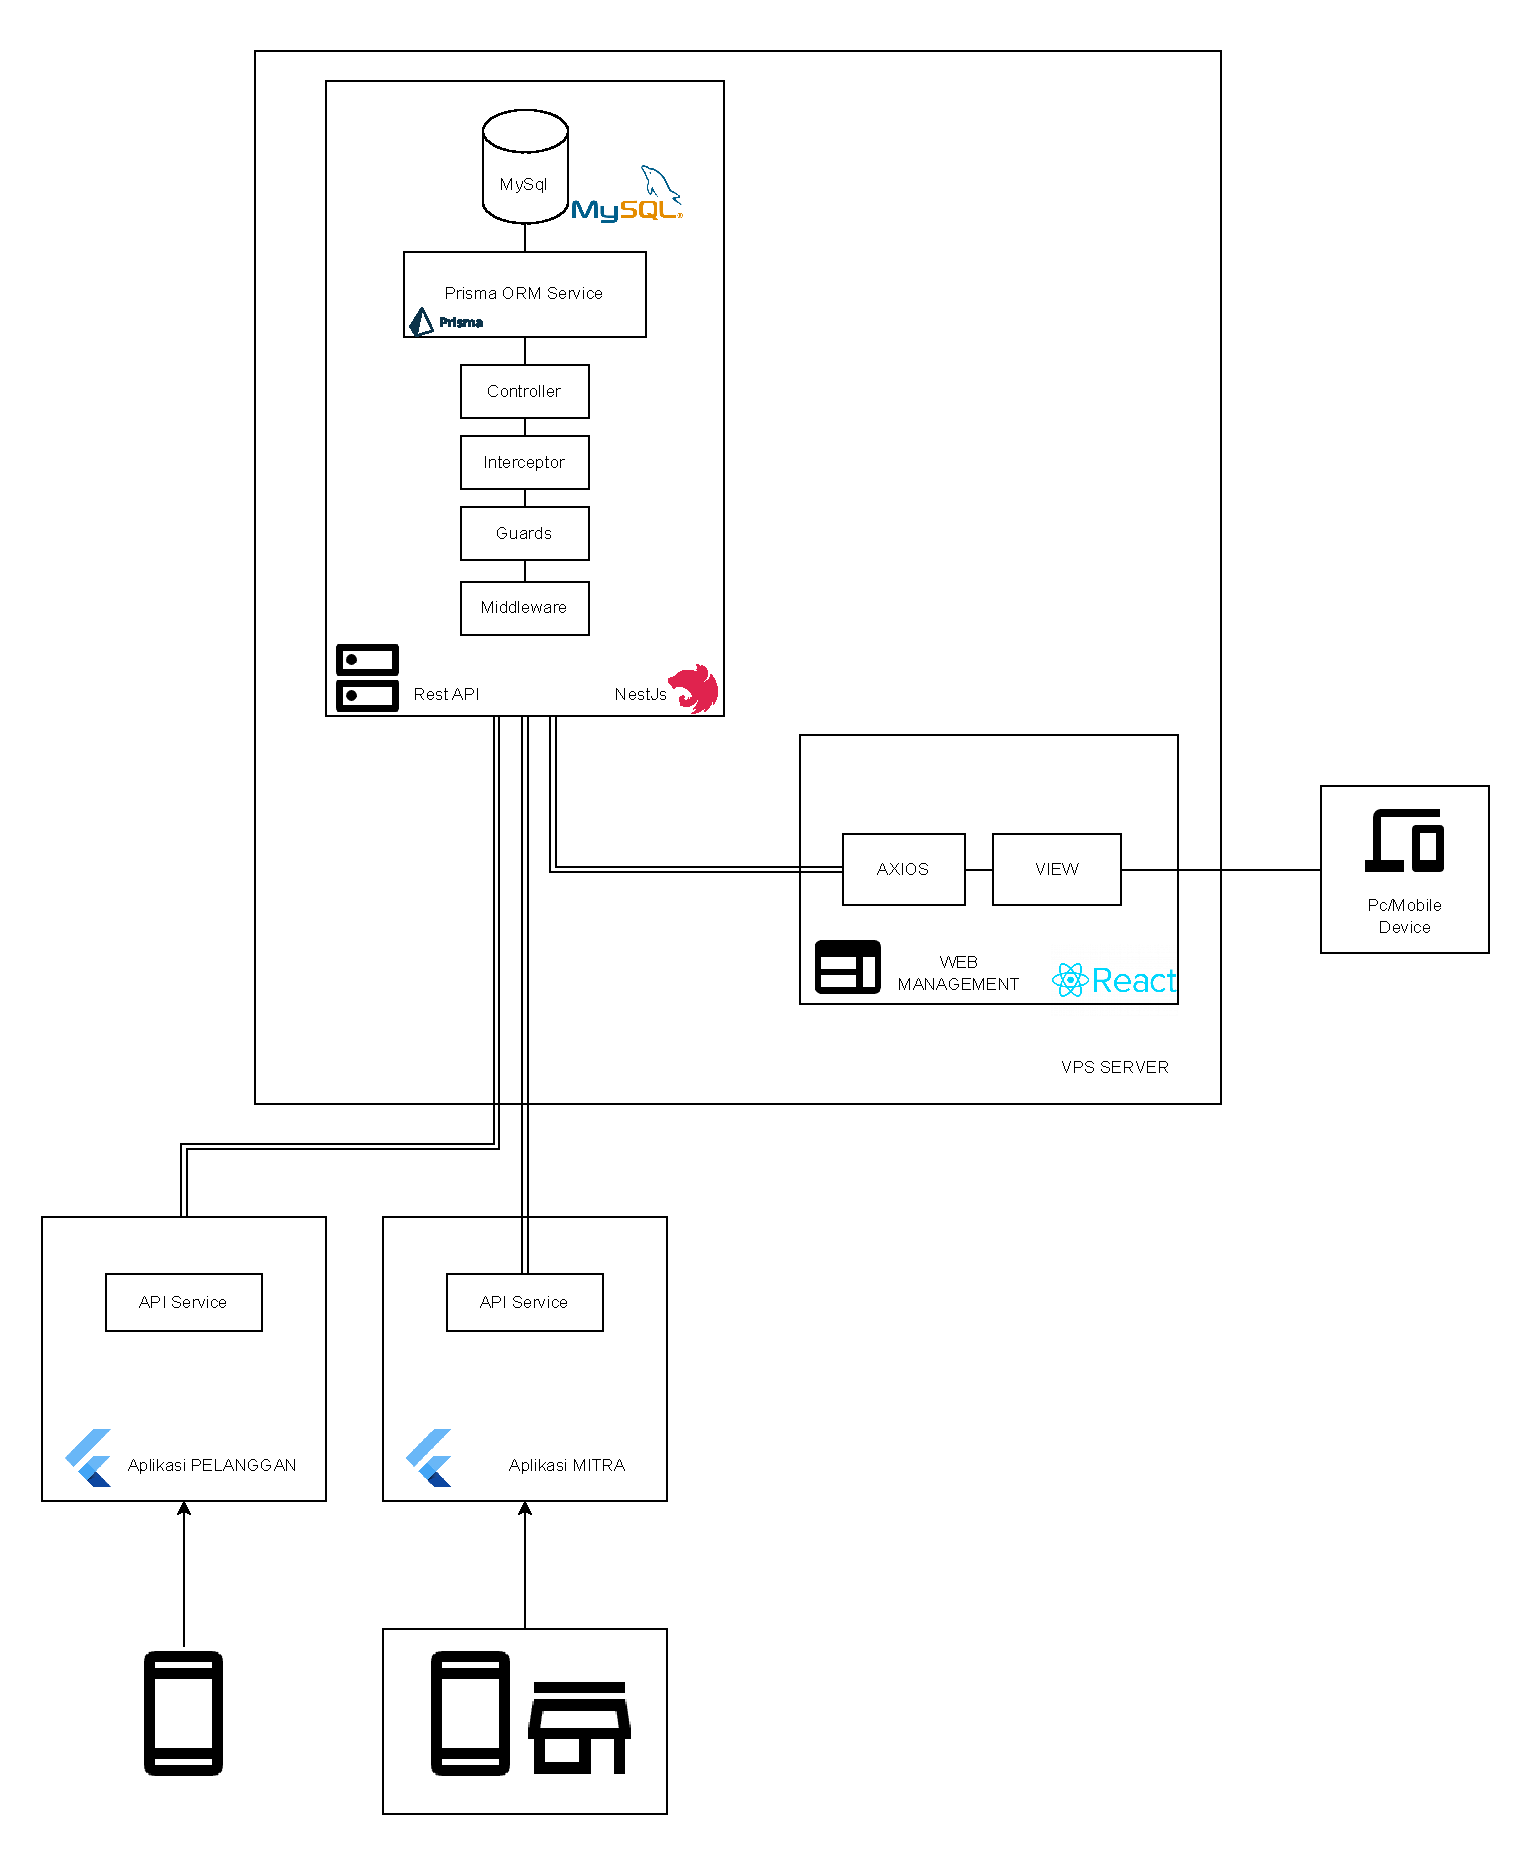
\includegraphics[width=0.73\textwidth]{drawio/System-Design-Architecture.drawio.pdf}
	\caption{Arsitektur Desain Sistem}
	\label{sistem-desain-arsitektur}
\end{figure}
\newpage
\subsection{Request Life Cycle}
Gambar \ref{sistem-desain} merupakan \textit{Request Lifecycle} yang menjelaskan management API atau bagaimana alur \textit{request} ditangani dari awal sampai akhir.
\begin{figure}[h]
	\centering
	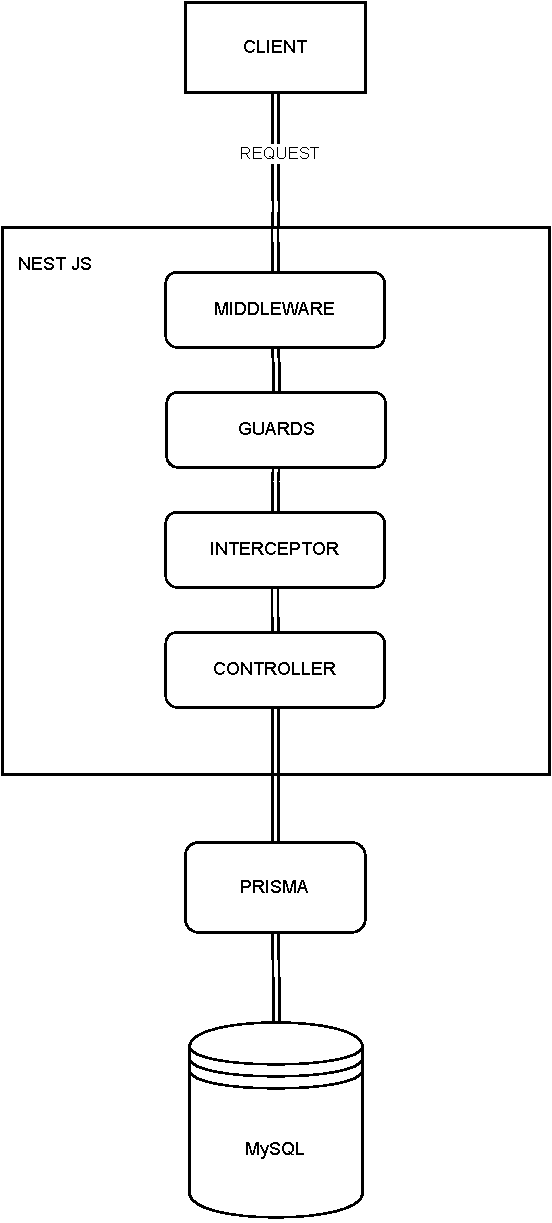
\includegraphics[width=0.35\textwidth]{drawio/sistem-desain.drawio.pdf}
	\caption{Desain Sistem}
	\label{sistem-desain}
\end{figure}
\subsubsection{Middleware}
Pada Middleware, fungsi akan dipanggil sebelum masuk ke routing. fungsi middleware dapat mengakses data \textit{request} dan \textit{response}. beberapa fungsi Middleware seperti \textit{logger}, dan cek notifikasi. Contoh penggunaan nya bisa dilihat pada listing \ref{lst:middleware}, request dapat di hentikan maupun di alihkan ke middleware selanjutnya.
\begin{lstlisting}[caption={Middleware},label={lst:middleware}]
  export class LoggerMiddleware implements NestMiddleware {
    use(req: Request, res: Response, next: NextFunction) {
      console.log('Request...');
      next();
    }
  }  
\end{lstlisting}

\subsubsection{Guard}
Pada Guard, \textit{request} akan dicek \textit{authenticity}, untuk mengetahui validitas dari \textit{request} tersebut. Tahap ini juga akan dicek keamanan session menggunakan JWT dan CSRF. Contoh penggunaan guard seperti pada listing \ref{lst:guard}, request yang menuju suatu controller akan di cek oleh guards, jika memiliki otorisasi maka akan dilanjutkan ke controller, jika tidak akan di reject dengan response forbidden access.
\begin{lstlisting}[caption={Penggunaan Guards pada Controller},label={lst:guard}]
  @UseGuards(AuthGuard)
  @Get('profile')
  getProfile(@Request() req) {
      return req.user;
  }
\end{lstlisting}


\subsubsection{Interceptor}
Setelah melalui Guard, Request akan masuk ke Interceptor. Dimana jika suatu \textit{request} mempunyai suatu karakteristik yang ditentukan, maka akan menjalankan fungsi tambahan. Interceptor terjadi ketika \textit{request} datang \textit{(pre)}, dan response \textit{(post)}. Contoh implementasi Interceptor terdapat pada listing \ref{lst:interceptor}.
\begin{lstlisting}[caption={Interceptor},label={lst:interceptor}]
  @UseInterceptors(FileInterceptor('profile_picture',fileInterceptor()))
  async update(@Param('id') id: string, @Body() data: Karyawan, @UploadedFile() file: Express.Multer.File): Promise<Karyawan> {}
\end{lstlisting}

\subsubsection{Controller}
Setelah melewati Interceptor, fungsi di Controller akan dijalankan. Jika pada Controller tersebut perlu data dari database maka akan turun ke service PrismaJs. Contoh karyawan controller pada listing \ref{lst:controller} dimana request akan diteruskan ke service setelah password di hash.
\begin{lstlisting}[caption={Controller},label={lst:controller}]
  @Controller('karyawan')
  @Post()
  async create(@Body() data: any): Promise<Karyawan> {
    const hashedPassword = await bcrypt.hash(data.password, 10);
    const karyawanData = { ...data, password: hashedPassword };
    return this.karyawanService.createKaryawan(karyawanData);
  }
\end{lstlisting}

\subsubsection{Service}
Pada Service, fungsi akan melakukan database call menggunakan ORM ke database MySQL yang akan di kembalikan (return) ker Controller\cite{NestJS}. Contoh implementasi service pada listing \ref{lst:service} dimana berfungsi untuk mengambil banyak karyawan.
\begin{lstlisting}[caption={Service},label={lst:service}]
  async karyawans(params: {
    skip?: number;
    take?: number;
    cursor?: Prisma.KaryawanWhereUniqueInput;
    where?: Prisma.KaryawanWhereInput;
    orderBy?: Prisma.KaryawanOrderByWithRelationInput;
  }): Promise<Karyawan[]> {
    const { skip, take, cursor, where, orderBy } = params;
    return this.prisma.karyawan.findMany({
      skip,take,cursor,where,orderBy,
    });
  }
\end{lstlisting}

\subsection{Persiapan}
Untuk memulai projek, ada beberapa tahap yang perlu dilakukan, pertama membuat projek nestjs menggunakan node, lalu dilanjutkan menginstall dependensi yang diperlukan

\subsubsection{Instalasi NestJS dan Prisma}
Hal pertama yang dilakukan untuk menginstall NestJS adalah membuka terminal lalu menjalankan command npm untuk menginstall NestJS, dilanjut dengan menginstall prisma client.
\begin{lstlisting}[caption={terminal: npm},label={lst:npm_install}]
  $ npm i -g @nestjs/cli
  $ nest new antria
  $ npm install prisma --save-dev
\end{lstlisting}
Command pada listing \ref{lst:npm_install} untuk melakukan generasi folder projek pada NestJS, dan menginstall prisma client sebagai dependensi. Prisma sendiri merupakan aplikasi CLI untuk membantu dalam manajemen database pada projek NestJS menggunakan ORM.

\subsubsection{Konfigurasi Prisma}
Berdasarkan SRS, didapatkan beberapa entity pada database meliputi: Pelanggan, Mitra, Produk, OrderList, Pesanan, Antrian, Karyawan, Review, Chat, dan Analytic. Implementasi juga harus sesuai dengan ERD (Entity Relationship Diagram) yang telah dibuat pada gambar \ref{erd}.
\begin{lstlisting}[caption={terminal: npx},label={lst:npx_prisma}]
  $ npx prisma init
  $ npx prisma migrate dev --name init
\end{lstlisting}
Command pada listing \ref{lst:npx_prisma} untuk inisialisasi prisma pada projek, berfungsi untuk generasi template config yang nanti harus diubah, seperti database connection dan database name nya.
Pada tahap ini juga penulis perlu mendefinisikan model dan relasi pada database ke bentuk notasi modelling prisma.
\begin{lstlisting}[caption={scheme.prisma},label={lst:scheme}]
  model Pesanan {
    invoice     String        @id
    payment     Payment
    pemesanan   OrderType?    @default(ONLINE)
    takeaway    Boolean       @default(false)
    status      PaymentStatus @default(PENDING)
    oderlist    OrderList[]
    pelanggan   Pelanggan     @relation(fields: [pelangganId], references: [id])
    pelangganId Int
    mitra       Mitra         @relation(fields: [mitraId], references: [id])
    mitraId     Int
    antrian     Antrian?
    antrianId   Int?
    created_at  DateTime      @default(now())
    updated_at  DateTime      @updatedAt
  }
  model OrderList {
    id        Int     @default(autoincrement()) @id
    quantity  Int     @default(1)
    note      String  @default("")
    pesanan   Pesanan @relation(fields: [pesananId], references: [invoice])
    produk    Produk  @relation(fields: [produkId], references: [id])
    produkId  Int
    pesananId String
  }
\end{lstlisting}
Pada listing \ref{lst:scheme} penulis mendefinisikan skema model pesanan dan model orderlist beserta relasi nya pada prisma. syntax @relation berguna untuk mendefinisikan relasi nya pada model.

\begin{figure}[p]
	\centering
	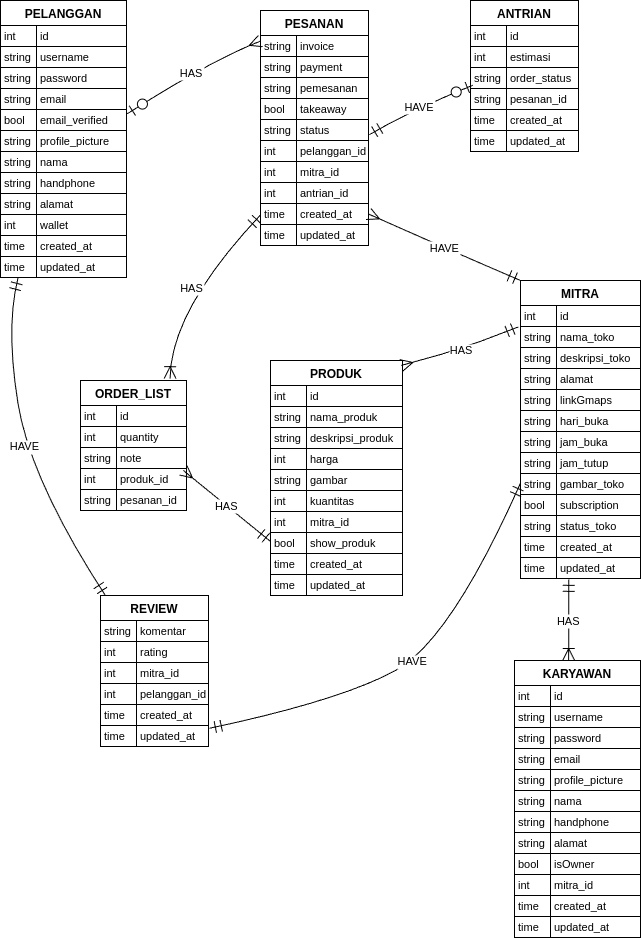
\includegraphics[width=1\textwidth]{drawio/erd.mermaid.png}
	\caption{Entity Relationship Diagram}
	\label{erd}
\end{figure}

\subsection{Implementasi}
\subsubsection{Guards}
implementasi code guards dibuat 2 fungsi, guards untuk pengguna, dan guards untuk mitra. Contoh implementasi pada listing \ref{lst:authguards}, disini penulis mendefinisikan guard untuk memeriksa JWT Token dari request yang diterima apakah valid.
\begin{lstlisting}[caption={Authentication Guards}, label={lst:authguards}]
  export class AuthGuard implements CanActivate {
    constructor(private jwtService: JwtService) {}
    async canActivate(context: ExecutionContext): Promise<boolean> {
      const request = context.switchToHttp().getRequest();
      const token = this.extractTokenFromHeader(request);
      if (!token) {
        throw new UnauthorizedException();
      }
      try {
        const payload = await this.jwtService.verifyAsync(
          token,
          {
            secret: jwtConstants.secret
          }
        );
        request['user'] = payload;
      } catch {
        throw new UnauthorizedException();
      }
      return true;
    }
  
    private extractTokenFromHeader(request: Request): string | undefined {
      const [type, token] = request.headers.authorization?.split(' ') ?? [];
      return type === 'Bearer' ? token : undefined;
    }
  }
\end{lstlisting}

\subsubsection{Interceptor}
Contoh implementasi terdapat pada listing \ref{lst:fileinterceptor}, dimana penulis mengimplementasikan interceptor untuk mendeteksi dan mengambil file dari multipart request data untuk diolah dan disimpan pada server.
\begin{lstlisting}[caption={File Interceptor},label={lst:fileinterceptor}]
  @UseInterceptors(FileInterceptor('profile_picture',{
    storage: diskStorage({
      destination: "./MediaUpload/",
      filename: (req, file, callback) => {
        const uniqueSuffix = uuidv4();
        const fileExtName = path.extname(file.originalname);
        const newFileName = `${uniqueSuffix}${fileExtName}`;
        callback(null, newFileName);
      }
    })
  }))
\end{lstlisting}

\subsubsection{Controller}
Controller minimal mengikuti banyak entity pada model. masing masing controller memiliki 4 fungsi yang merepresentasikan method http yaitu GET, POST, PUT, DELETE. Khusus untuk endpoint DELETE, pada beberapa cotroller data tidak secara langsung di delete, namun hanya diubah status nya dari enabled ke disabled.
\begin{enumerate}
  \item Pelanggan controller
  \item Mitra controller
  \item Produk controller
  \item OrderList controller
  \item Pesanan controller
  \item Antrian controller
  \item Karyawan controller
  \item Review controller
  \item Analytic controller
\end{enumerate}

\subsubsection{Service}
Sama seperti controller, banyak service minimal mengikuti banyak entity pada model.
bedanya service berinteraksi langsung dengan ORM Prisma.
\begin{enumerate}
  \item Pelanggan Service
  \item Mitra Service
  \item Produk Service
  \item OrderList Service
  \item Pesanan Service
  \item Antrian Service
  \item Karyawan Service
  \item Review Service
  \item Analytic Service
\end{enumerate}

\subsubsection{API Endpoint}
Untuk menghindari Anti Pattern, API endpoint sesuai dengan nama entity pada model.
setiap endpoint entity mendukung 4 method http yaitu POST, GET, PUT, dan DELETE.
\begin{enumerate}
  \item Auth Endpoint,
  Tabel \ref{tbl:auth} memetakan controller auth pada endpoint REST API.
  \begin{longtable}{| p{3.5cm} | p{1.5cm} | p{8cm} |}
    \caption{Auth Endpoint Table} \label{tbl:auth} \\
    \hline
    \textbf{Path} & \textbf{Method} & \textbf{Description} \\
    \hline
    \endfirsthead
    
    \multicolumn{3}{c}%
    {{\bfseries \tablename\ \thetable{} -- continued from previous page}} \\
    \hline
    \textbf{Path} & \textbf{Method} & \textbf{Description} \\
    \hline
    \endhead
    
    \hline \multicolumn{3}{|r|}{{Continued on next page}} \\ \hline
    \endfoot
    
    \hline
    \endlastfoot
    
    /auth/login/pelanggan & POST  & Endpoint untuk aplikasi mobile pelanggan, pengguna memasukkan credential login lalu akan mendapatkan JWT Token untuk mengakses enpoint API lain nya \\
    \hline
    /auth/login/mitra & POST & Endpoint untuk aplikasi mobile mitra, dan Web Dashboard. pengguna memasukkan credential login lalu akan mendapatkan JWT Token untuk mengakses enpoint API lain nya \\
    \hline
    /auth/profile & GET  & Endpoint untuk decode JWT payload \\
    \hline
    
  \end{longtable}

  \item Pelanggan Endpoint,
  Tabel \ref{tbl:pelanggan} memetakan controller pelanggan pada endpoint REST API.
  \begin{longtable}{| p{2.5cm} | p{1.5cm} | p{9cm} |}
    \caption{Pelanggan Endpoint Table} \label{tbl:pelanggan} \\
    \hline
    \textbf{Path} & \textbf{Method} & \textbf{Description} \\
    \hline
    \endfirsthead
    
    \multicolumn{3}{c}%
    {{\bfseries \tablename\ \thetable{} -- continued from previous page}} \\
    \hline
    \textbf{Path} & \textbf{Method} & \textbf{Description} \\
    \hline
    \endhead
    
    \hline \multicolumn{3}{|r|}{{Continued on next page}} \\ \hline
    \endfoot
    
    \hline
    \endlastfoot
    
    /pelanggan & GET  & Endpoint untuk mengambil seluruh pelanggan terdaftar pada aplikasi \\
    \hline
    /pelanggan & POST  & Endpoint untuk membuat akun pelanggan baru \\
    \hline
    /pelanggan/\{id\} & GET  & Endpoint untuk mengambil akun pelanggan dengan id tertentu \\
    \hline
    /pelanggan/\{id\} & PUT  & Endpoint untuk memperbarui akun pelanggan dengan id tertentu \\
    \hline
    /pelanggan/\{id\} & DELETE  & Endpoint untuk menghapus (disable) akun pelanggan dengan id tertentu \\
    \hline
    
  \end{longtable}
  \item Karyawan Endpoint,
  Tabel \ref{tbl:karyawan} memetakan controller karyawan pada endpoint REST API.
  \begin{longtable}{| p{4.5cm} | p{1.5cm} | p{7cm} |}
    \caption{Karyawan Endpoint Table} \label{tbl:karyawan} \\
    \hline
    \textbf{Path} & \textbf{Method} & \textbf{Description} \\
    \hline
    \endfirsthead
    
    \multicolumn{3}{c}%
    {{\bfseries \tablename\ \thetable{} -- continued from previous page}} \\
    \hline
    \textbf{Path} & \textbf{Method} & \textbf{Description} \\
    \hline
    \endhead
    
    \hline \multicolumn{3}{|r|}{{Continued on next page}} \\ \hline
    \endfoot
    
    \hline
    \endlastfoot
    
    /karyawan & GET  & Endpoint untuk mengambil seluruh karyawan terdaftar pada aplikasi \\
    \hline
    /karyawan & POST  & Endpoint untuk membuat akun karyawan baru \\
    \hline
    /karyawan/\{id\} & GET  & Endpoint untuk mengambil akun karyawan dengan id tertentu \\
    \hline
    /karyawan/\{id\} & PUT  & Endpoint untuk memperbarui akun karyawan dengan id tertentu \\
    \hline
    /karyawan/\{id\} & DELETE  & Endpoint untuk menghapus (disable) akun karyawan dengan id tertentu \\
    \hline
    /karyawan/mitra/\{mitraId\} & GET  & Endpoint untuk mengambil seluruh karyawan terdaftar pada aplikasi dan id mitra tertentu \\
    \hline
    
  \end{longtable}

  \item Mitra Endpoint,
  Tabel \ref{tbl:mitra} memetakan controller mitra pada endpoint REST API.
  \begin{longtable}{| p{2cm} | p{1.5cm} | p{9.5cm} |}
    \caption{Mitra Endpoint Table} \label{tbl:mitra} \\
    \hline
    \textbf{Path} & \textbf{Method} & \textbf{Description} \\
    \hline
    \endfirsthead
    
    \multicolumn{3}{c}%
    {{\bfseries \tablename\ \thetable{} -- continued from previous page}} \\
    \hline
    \textbf{Path} & \textbf{Method} & \textbf{Description} \\
    \hline
    \endhead
    
    \hline \multicolumn{3}{|r|}{{Continued on next page}} \\ \hline
    \endfoot
    
    \hline
    \endlastfoot
    
    /mitra & GET  & Endpoint untuk mengambil seluruh mitra terdaftar pada aplikasi \\
    \hline
    /mitra & POST  & Endpoint untuk membuat akun mitra baru \\
    \hline
    /mitra/\{id\} & GET  & Endpoint untuk mengambil mitra dengan id tertentu \\
    \hline
    /mitra/\{id\} & PUT  & Endpoint untuk mengaupdate mitra dengan id tertentu \\
    \hline
    /mitra/\{id\} & DELETE  & Endpoint untuk menghapus (disable) mitra dengan id tertentu \\
    \hline
    
  \end{longtable}

  \item Produk Endpoint,
  Tabel \ref{tbl:produk} memetakan controller prduk pada endpoint REST API.
  \begin{longtable}{| p{3.5cm} | p{1.5cm} | p{8cm} |}
    \caption{Produk Endpoint Table} \label{tbl:produk} \\
    \hline
    \textbf{Path} & \textbf{Method} & \textbf{Description} \\
    \hline
    \endfirsthead
    
    \multicolumn{3}{c}%
    {{\bfseries \tablename\ \thetable{} -- continued from previous page}} \\
    \hline
    \textbf{Path} & \textbf{Method} & \textbf{Description} \\
    \hline
    \endhead
    
    \hline \multicolumn{3}{|r|}{{Continued on next page}} \\ \hline
    \endfoot
    
    \hline
    \endlastfoot
    
    /produk & GET  & Endpoint untuk mengambil seluruh produk yang terdaftar pada aplikasi \\
    \hline
    /produk & POST  & Endpoint untuk membuat produk baru pada mitra tertentu \\
    \hline
    /produk/\{id\} & GET  & Endpoint untuk mengambil prduk dengan id tertentu \\
    \hline
    /produk/\{id\} & PUT  & Endpoint untuk memperbarui produk dengan id tertentu \\
    \hline
    /produk/\{id\} & DELETE  & Endpoint untuk menghapus (disable) produk dengan id tertentu \\
    \hline
    /produk/mitra/\{mitraId\} & GET  & Endpoint untuk mengambil produk dari id mitra tertentu \\
    \hline
    
  \end{longtable}

  \item Pesanan Endpoint,
  Tabel \ref{tbl:pesanan} memetakan controller pesanan pada endpoint REST API.
  \begin{longtable}{| p{4cm} | p{1.5cm} | p{7.5cm} |}
    \caption{Pesanan Endpoint Table} \label{tbl:pesanan} \\
    \hline
    \textbf{Path} & \textbf{Method} & \textbf{Description} \\
    \hline
    \endfirsthead
    
    \multicolumn{3}{c}%
    {{\bfseries \tablename\ \thetable{} -- continued from previous page}} \\
    \hline
    \textbf{Path} & \textbf{Method} & \textbf{Description} \\
    \hline
    \endhead
    
    \hline \multicolumn{3}{|r|}{{Continued on next page}} \\ \hline
    \endfoot
    
    \hline
    \endlastfoot
    
    /pesanan & GET  & Endpoint untuk mengambil seluruh pesanan \\
    \hline
    /pesanan & POST  & Endpoint untuk membuat pesanan baru \\
    \hline
    /pesanan/\{invoice\} & GET  & Endpoint untuk mengambil pesanan dengan invoice tertentu \\
    \hline
    /pesanan/\{invoice\} & PUT  & Endpoint untuk memperbarui pesanan dengan invoice tertentu \\
    \hline
    /pesanan/\{invoice\} & DELETE  & Endpoint untuk menghapus (disable) pesanan dengan invoice tertentu \\
    \hline
    /pesanan/mitra/\{mitraId\} & GET  & Endpoint untuk mengambil seluruh pesanan dari id mitra tertentu \\
    \hline
    
  \end{longtable}

  \item OrderList Endpoint,
  Tabel \ref{tbl:orderlist} memetakan controller orderlist pada endpoint REST API.
  \begin{longtable}{| p{4cm} | p{1.5cm} | p{7.5cm} |}
    \caption{OrderList Endpoint Table} \label{tbl:orderlist} \\
    \hline
    \textbf{Path} & \textbf{Method} & \textbf{Description} \\
    \hline
    \endfirsthead
    
    \multicolumn{3}{c}%
    {{\bfseries \tablename\ \thetable{} -- continued from previous page}} \\
    \hline
    \textbf{Path} & \textbf{Method} & \textbf{Description} \\
    \hline
    \endhead
    
    \hline \multicolumn{3}{|r|}{{Continued on next page}} \\ \hline
    \endfoot
    
    \hline
    \endlastfoot
    
    /orderlist & POST  & Endpoint untuk membuat orderlist baru\\
    \hline
    /orderlist/\{id\} & GET  & Endpoint untuk mengambil orderlist dengan id tertentu\\
    \hline
    /orderlist/\{id\} & PUT  & Endpoint untuk memperbarui orderlist dengan id tertentu\\
    \hline
    /orderlist/\{id\} & DELETE  & Endpoint untuk menghapus (disable) orderlist dengan id tertentu\\
    \hline
    /orderlist/invoice/\{invoice\} & GET  & Endpoint untuk mengambil orderlist dengan invoice pesanan tertentu\\
    \hline
    
  \end{longtable}

  \item Antrian Endpoint,
  Tabel \ref{tbl:antrian} memetakan controller antrian pada endpoint REST API.
  \begin{longtable}{| p{4cm} | p{1.5cm} | p{7.5cm} |}
    \caption{Antrian Endpoint Table} \label{tbl:antrian} \\
    \hline
    \textbf{Path} & \textbf{Method} & \textbf{Description} \\
    \hline
    \endfirsthead
    
    \multicolumn{3}{c}%
    {{\bfseries \tablename\ \thetable{} -- continued from previous page}} \\
    \hline
    \textbf{Path} & \textbf{Method} & \textbf{Description} \\
    \hline
    \endhead
    
    \hline \multicolumn{3}{|r|}{{Continued on next page}} \\ \hline
    \endfoot
    
    \hline
    \endlastfoot
    
    /antrian & POST  & Endpoint untuk membuat antrian baru \\
    \hline
    /antrian/\{id\} & GET  & Endpoint untuk mengambil antrian dengan id tertentu \\
    \hline
    /antrian/\{id\} & PUT  & Endpoint untuk memperbarui antrian dengan id tertentu \\
    \hline
    /antrian/\{id\} & DELETE  &  Endpoint untuk menghapus (disable) antrian dengan id tertentu \\
    \hline
    /antrian/mitra/\{mitraId\} & GET  & Endpoint untuk mengambil antrian pada mitra tertentu \\
    \hline
    
  \end{longtable}

  \item Reviews Endpoint,
  Tabel \ref{tbl:review} memetakan controller review pada endpoint REST API.
  \begin{longtable}{| p{5cm} | p{1.5cm} | p{6.5cm} |}
    \caption{Reviews Endpoint Table} \label{tbl:review} \\
    \hline
    \textbf{Path} & \textbf{Method} & \textbf{Description} \\
    \hline
    \endfirsthead
    
    \multicolumn{3}{c}%
    {{\bfseries \tablename\ \thetable{} -- continued from previous page}} \\
    \hline
    \textbf{Path} & \textbf{Method} & \textbf{Description} \\
    \hline
    \endhead
    
    \hline \multicolumn{3}{|r|}{{Continued on next page}} \\ \hline
    \endfoot
    
    \hline
    \endlastfoot
    /reviews & GET  & Endpoint untuk mengambil seluruh review \\
    \hline
    /reviews & POST  & Endpoint untuk membuat review baru \\
    \hline
    /reviews/mitra/\{mitraId\} & GET  & Endpoint untuk mengambil review pada mitra tertentu \\
    \hline
    /reviews/\{mitraId\}/\{pelangganId\} & GET  & Endpoint untuk mengambil review pelanggan pada mitra tertentu \\
    \hline
    /reviews/\{mitraId\}/\{pelangganId\} & PUT  & Endpoint untuk memperbarui review pelanggan pada mitra tertentu \\
    \hline
    /reviews/\{mitraId\}/\{pelangganId\} & DELETE  & Endpoint untuk menghapus review pelanggan pada mitra tertentu\\
    \hline
    
  \end{longtable}

  \item Image server endpoint,
  endpoint pada tabel \ref{tbl:imageserver} untuk menyajikan gambar ke client melalui REST API.
  \begin{longtable}{| p{3cm} | p{1.5cm} | p{8.5cm} |}
    \caption{Image server Endpoint Table} \label{tbl:imageserver} \\
    \hline
    \textbf{Path} & \textbf{Method} & \textbf{Description} \\
    \hline
    \endfirsthead
    
    \multicolumn{3}{c}%
    {{\bfseries \tablename\ \thetable{} -- continued from previous page}} \\
    \hline
    \textbf{Path} & \textbf{Method} & \textbf{Description} \\
    \hline
    \endhead
    
    \hline \multicolumn{3}{|r|}{{Continued on next page}} \\ \hline
    \endfoot
    
    \hline
    \endlastfoot
    /image/\{fileName\} & GET  & Endpoint untuk menampilkan gambar dengan filename tertentu\\
    \hline
    
  \end{longtable}
\end{enumerate}

\subsection{Kesesuaian dengan Functional Requirement}

\subsection{Alur Pengujian}
Pengujian menggunakan metode white box testing yaitu unit testing. Testing dilakukan pada setiap fungsi yang telah dibuat tanpa terhubung ke komponen lain. Setelah semua fungsi lulus unit testing, dilakukan performance dan load testing menggunakan library K6 pada node.js untuk mnegukur performansi aplikasi. Environment Testing menggunakan lokal build pada laptop penulis dan menggunakan tunnelling Cloudflare untuk mengukur performa network dan cpu load nya. Diagram alur pengujian dapat dilihat pada gambar \ref{alur-testing}.

\begin{figure}[h]
	{\centering {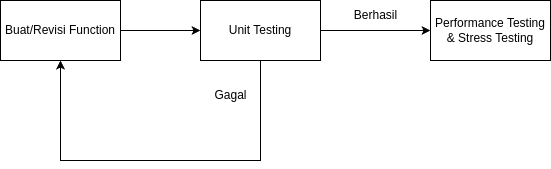
\includegraphics[scale=0.75]{drawio/alur-testing.png}}\par}
	\caption{Alur Testing}
	\label{alur-testing}
\end{figure}

\subsubsection{Unit Testing}
Pengujian dimulai dengan membuat file yang bernama <component>.spec.ts seperti terlihat pada gambar \ref{ut1}. Lalu pada file tersebut penulis mendeskripsikan test apa yang akan dibuat seperti contoh pada listing \ref{lst:jest-testing}, pertama difinisikan parameter yang diperlukan function lalu expect hasil keluaran fungsi sesuai dengan yang ditentukan.
\begin{figure}[h]
	{\centering {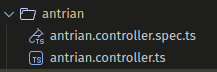
\includegraphics[scale=1]{drawio/unit-testing1.png}}\par}
	\caption{File spec.ts}
	\label{ut1}
\end{figure}

\begin{lstlisting}[caption={Contoh Testing Menggunakan Jest},label={lst:jest-testing}]
  describe('canActivate', () => {
  it('should return true if user role is karyawan', async () => {
    const mockRequest = { user: { role: 'karyawan' } };
    const mockContext = { switchToHttp: () => ({ getRequest: () => mockRequest }) } as unknown as ExecutionContext;

    expect(await guard.canActivate(mockContext)).toBe(true);
  });

  it('should return false if user role is not karyawan', async () => {
    const mockRequest = { user: { role: 'admin' } };
    const mockContext = { switchToHttp: () => ({ getRequest: () => mockRequest }) } as unknown as ExecutionContext;

    expect(await guard.canActivate(mockContext)).toBe(false);
  });
});
\end{lstlisting}

\subsubsection{Performance Testing \& Stress Testing}
Pengujian performa dilakukan menggunakan K6 dengan cara melakukan request secara konkuren berdasarkan VU (Virtual User) yang di spesifikasikan. Pada listing \ref{lst:k6-thresh}, penulis mendefinisikan VU sebanyak 10, dengan stages pada detik 10 harus terdapat 100 VU yang melakukan, dan detik 20 terdapat 200 VU yang melakukan request, ini mengakibatkan fungsi akan menambah VU secara dinamis dalam 1 testing. Penulis juga mendefinisikan Request blocked tidak boleh lebih dari 30 milisecond, request connecting tidak boleh selama 100 milisecond untuk 90\% request, durasi request tidak lebih dari 1 detik untuk 90\% request, dan rate kegagalan request kurang dari 0,1\% \cite{nah2004study}.
\begin{lstlisting}[caption={Konfigurasi dan threshold yang perlu dicapai pada K6},label={lst:k6-thresh}]
  export const options = {
    vus: 10,
    thresholds: {
      http_req_blocked: ['p(100)<=30'],
      http_req_connecting: ['p(90)<100'],
      http_req_duration: ['p(90)<1000'],
      http_req_failed: ['rate<0.1'],
      http_req_receiving: ['p(90)<50'],
      http_req_sending: ['p(90)<10'],
    },
    tags: {
      environment: 'production',
    },
    stages: [
      { duration: '10s', target: 100 },
      { duration: '20s', target: 200 },
    ],
  };
\end{lstlisting}

\newpage

\subsection{Deployment}
Ketika backend selesai di kembangkan dan siap dipakai maka akan dilakukan deployment.
Pada diagram \ref{deployment} menjelaskan bagaimana server backend berkomunikasi dengan Aplikasi lain melalui protokol HTTPS dan memiliki database pusat yaitu di backend untuk sinkronisasi data dari satu aplikasi ke aplikasi lain. 

\begin{figure}[h]
	{\centering {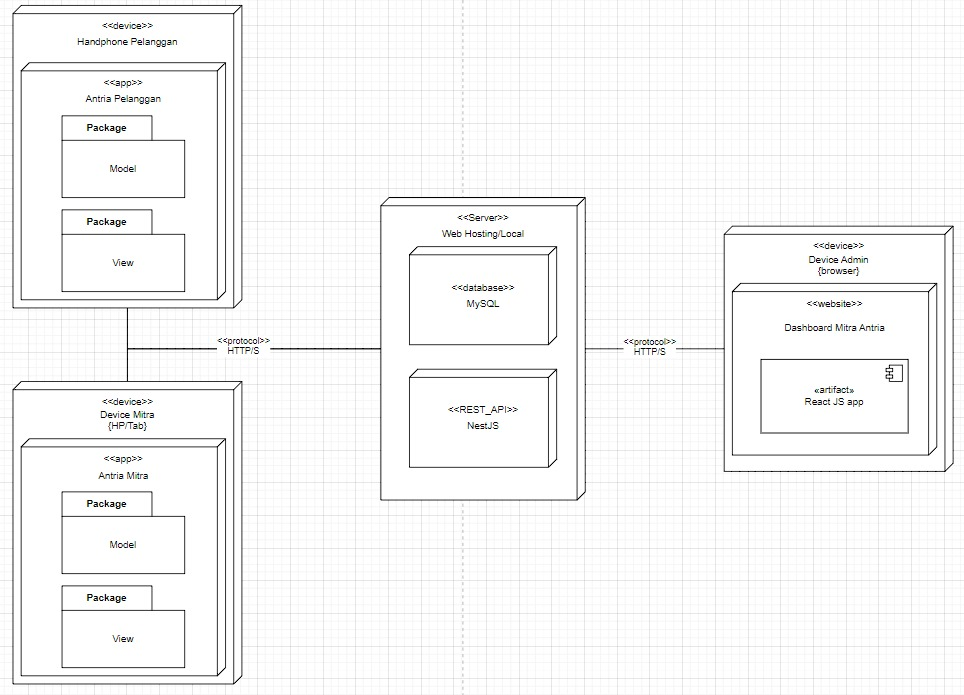
\includegraphics[scale=0.6]{drawio/deployment.jpg}}\par}
	\caption{Deployment Diagram}
	\label{deployment}
\end{figure}

\newpage

\section{Evaluasi}

\subsection{Hasil Pengujian}
\subsubsection{Unit Testing}
 Untuk unit testing, terdapat 2 Test suite pada setiap entity kecuali auth dimana auth memiliki 3 test suite yang ditotal sebanyak 21 test suite yang perlu dibuat dan dilakukan.

\begin{figure}[h]
	{\centering {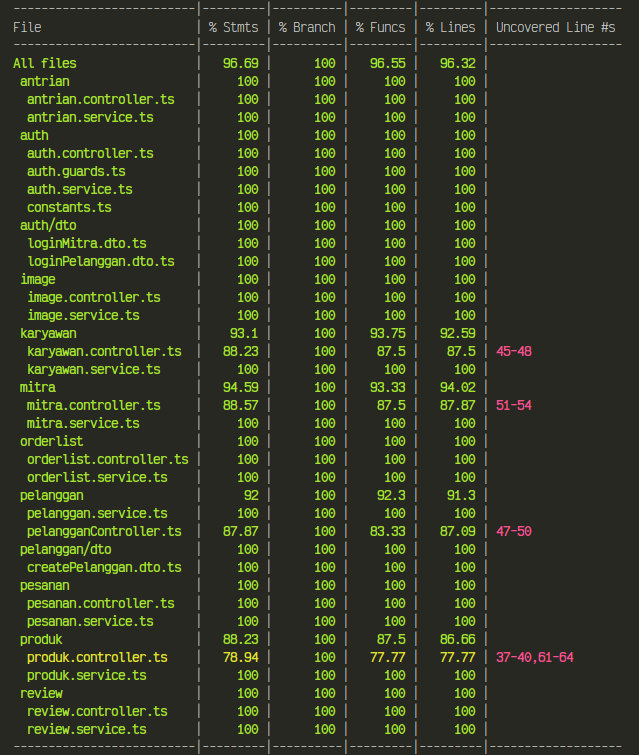
\includegraphics[scale=0.8]{drawio/unitTesting.png}}\par}
	\caption{Hasil unit testing menggunakan jest}
	\label{unit-testing}
\end{figure}

\begin{figure}[h]
	{\centering {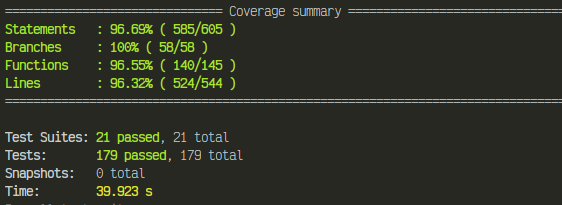
\includegraphics[scale=0.9]{drawio/CoverageSummary.png}}\par}
	\caption{Coverage Summary}
	\label{coverage-summary}
\end{figure}

\newpage

\subsubsection{Performance Testing}
Pada bagian performance testing, saya menguji beberapa fitur yang mewakili method HTTP GET, POST, dan PUT. Untuk GET saya menguji fungsi untuk mengambil seluruh mitra, untuk POST saya menguji fungsi untuk Register user, untuk PUT saya menguji fungsi update user.

\begin{figure}[H]
	{\centering {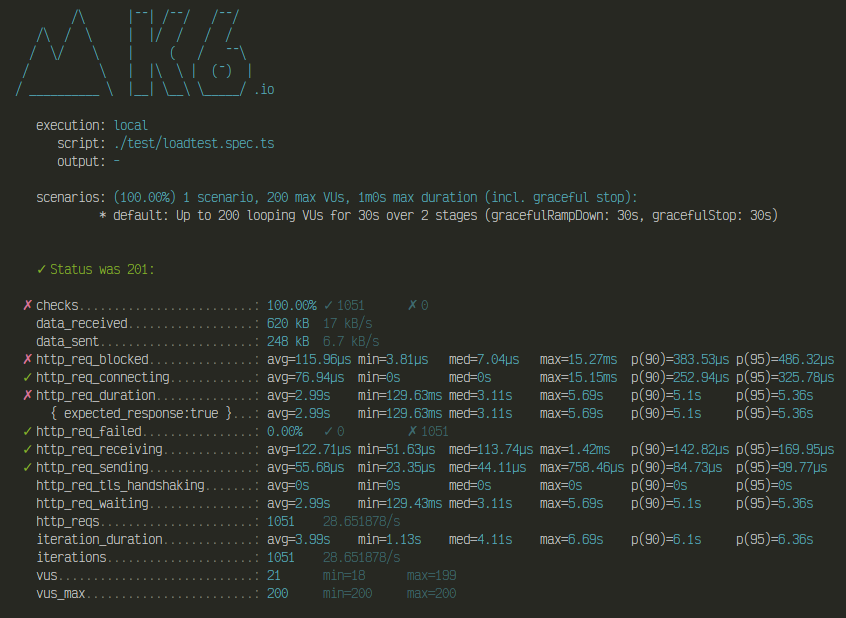
\includegraphics[scale=0.65]{drawio/register-test.png}}\par}
	\caption{Hasil performance testing untuk register user (POST)}
	\label{register-testing}
\end{figure}

\begin{figure}[H]
	{\centering {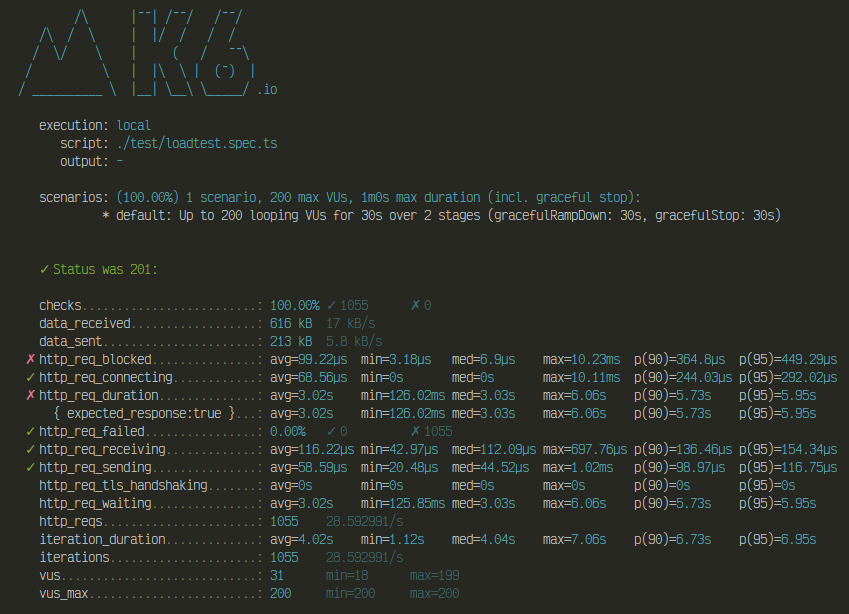
\includegraphics[scale=0.65]{drawio/login-test.png}}\par}
	\caption{Hasil performance testing untuk login user (POST)}
	\label{login-testing}
\end{figure}

\begin{figure}[H]
	{\centering {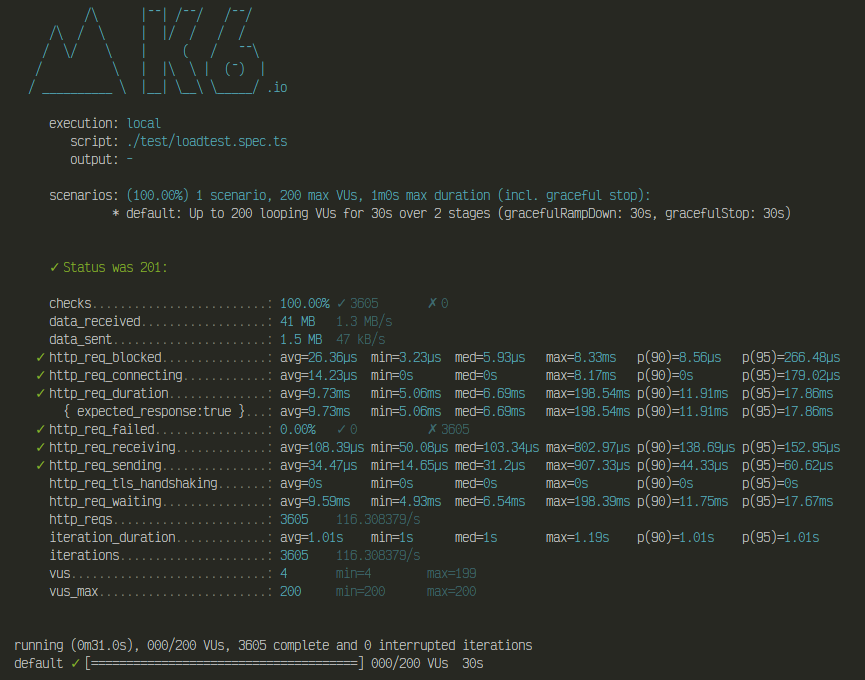
\includegraphics[scale=0.65]{drawio/mitra-test.png}}\par}
	\caption{Hasil performance testing get semua mitra (GET)}
	\label{mitra-testing}
\end{figure}

\begin{figure}[H]
	{\centering {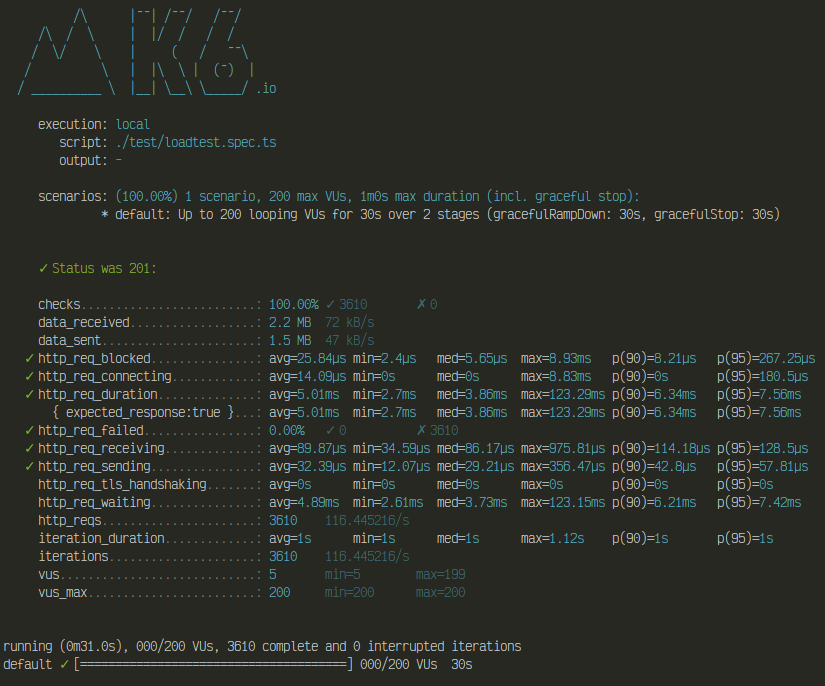
\includegraphics[scale=0.6]{drawio/mitra-id-test.png}}\par}
	\caption{Hasil performance testing get mitra berdasar id (GET)}
	\label{mitra-id-testing}
\end{figure}

\begin{figure}[H]
	{\centering {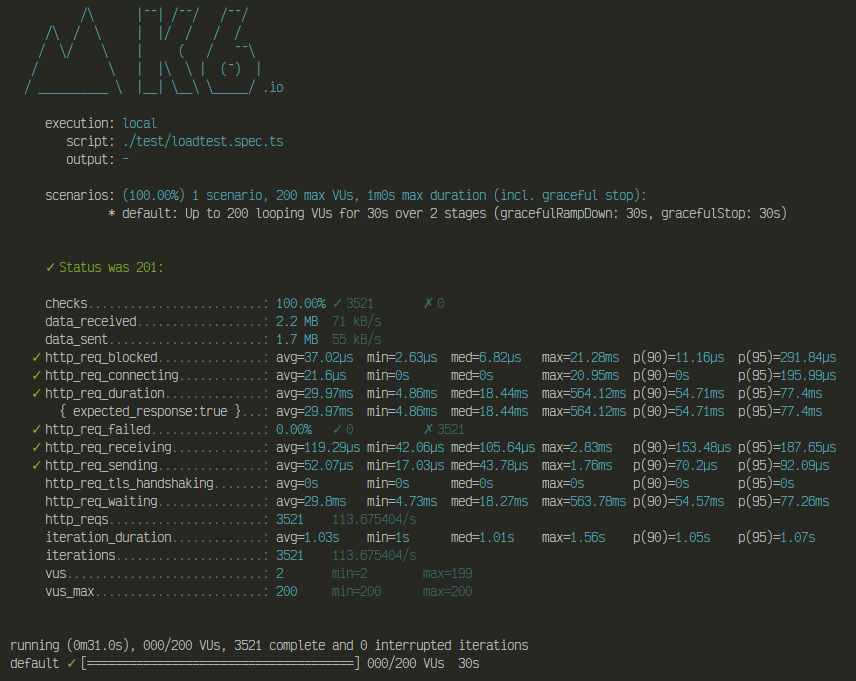
\includegraphics[scale=0.6]{drawio/update-user-test.png}}\par}
	\caption{Hasil performance testing update user berdasar id (PUT)}
	\label{update-user-testing}
\end{figure}

\newpage


\subsection{Analisis Hasil Pengujian}
\subsubsection{Unit Testing}
Semua test case pada unit testing lolos uji atau pass dengan code coverage 96,32\% dengan LOC (Line Of Code) sekitar 524 dari 544 LOC. Jika dilihat pada gambar \ref{unit-testing} LOC yang tidak teruji terdapat pada file karyawan, mitra, pelanggan, dan produk. Kode yang tidak teruji berupa interceptor untuk mendeteksi file gambar pada multipart request, fungsi tersebut tidak dapat diuji pada unit testing dikarenakan perlunya request autentik multipart dan tidak bisa di simulasikan secara efektif.

\subsubsection{Performance Testing}
Performance testing berfungsi untuk melihat seberapa kuat backend untuk melayani banyak request dalam secara bersamaan. Dilihat dari hasil testing ada beberapa hal yang ditemukan. Dari 5 Testing, 2 diantaranya belum memenuhi spesifikasi yang telah ditetapkan. Pada gambar \ref{login-testing} menampilkan hasil testing dari fungsi login user. Tertulis rata rata durasi sebesar 3 detik dengan delay terendah berada di 126 milisecond dan delay tertinggi berada di 6 detik, hal ini diakibatkan oleh fungsi login yang membanding satu string password dengan versi bcrypt, dengan cara string password di enkripsi terlebih dahulu lalu di bandingkan, hal ini memakan waktu yang mengakibatkan delay tinggi saat server over capacity. Lalu pada gambar \ref{register-testing} memiliki hasil yang mirip dengan fungsi login, hal ini dikarenakan fungsi register melakukan insert database dimana pada orm Prisma sedikit lebih lambat dibanding edit dan view data. Pada fungsi get all mitra pada gambar \ref{mitra-testing}, rata-rata delay yang didapatkan tidak lambat yaitu sebesar 9,7 milisecond, sedangkan untuk get mitra by id pada gambar \ref{mitra-id-testing} sebesar 5 milisecond. Untuk fungsi terakhir yaitu update user by id pada gambar \ref{update-user-testing}, rata-rata duration yang di dapat sebesar 30 milisecond.


\section{Kesimpulan}

Berdasarkan implementasi dan perancangan sistem menggunakan NestJs dan Prisma, dapat diambil beberapa kesimpulan terkait Anti Pattern, Keamanan, Maintainabilitas, dan Performa.
\begin{enumerate}
  \item \textbf{Anti Pattern}\newline
  Penting untuk menghindari Anti Pattern dalam pengembangan aplikasi, yaitu praktik yang tidak dianjurkan atau kesalahan umum yang sering dilakukan. Dalam sistem yang dikembangkan, beberapa langkah yang diambil untuk menghindari Anti Pattern meliputi:
  \begin{itemize}
    \item \textbf{Consistent Endpoint Naming}: Penamaan endpoint mengikuti nama entity pada model, sehingga memudahkan pengembangan dan pemahaman API.
    \item \textbf{Separation of Concerns}: Memisahkan setiap komponen dalam aplikasi (Middleware, Guards, Interceptor, Controller, dan Service) sesuai dengan tanggung jawab masing-masing.
    \item \textbf{Avoiding Over-fetching and Under-fetching}: Endpoint API dirancang untuk menghindari pengambilan data yang berlebihan atau kurang, sesuai dengan kebutuhan aplikasi.
  \end{itemize}
  \item \textbf{keamanan}\newline
  Keamanan adalah aspek penting dalam pengembangan aplikasi, beberapa langkah yang diambil untuk memastikan keamanan sistem meliputi:
  \begin{itemize}
    \item \textbf{JWT Authentication}: Penggunaan JWT untuk otentikasi dan otorisasi pengguna, memastikan hanya pengguna yang valid dapat mengakses endpoint tertentu.
    \item \textbf{Data Validation}: Validasi data pada setiap layer (Controller, Service) untuk memastikan integritas dan keamanan data.
    \item \textbf{Encryption}: Penggunaan bcrypt untuk meng-hash password pengguna sebelum disimpan di database.
  \end{itemize}
  \item \textbf{Maintainabilitas}\newline
  Maintainabilitas adalah kemampuan sistem untuk dapat dipelihara dan dikembangkan lebih lanjut dengan mudah dengan cara menggunakan Prisma sebagai ORM untuk manajemen database yang lebih mudah dan terstruktur.
\end{enumerate}

\subsection{Saran}
Untuk meningkatkan performa dan skalabilitas sistem, terdapat beberapa hal yang perlu diperhatikan dan ditingkatkan, antara lain:
\begin{enumerate}
  \item \textbf{Performa} \newline
  \begin{itemize}
    \item \textbf{Optimasi Query Database}: Lakukan analisis dan optimasi query yang digunakan untuk memastikan performa yang lebih baik. Penggunaan indeks yang tepat pada tabel-tabel penting dapat meningkatkan kecepatan akses data.
    \item \textbf{Implementasi Caching yang Lebih Lanjut}: Integrasikan mekanisme caching yang lebih canggih, seperti Redis, untuk menyimpan hasil query yang sering digunakan dan mengurangi beban pada database.
    \item \textbf{Profiling dan Monitoring}: Gunakan alat profiling dan monitoring untuk mengidentifikasi dan memperbaiki bottleneck dalam aplikasi. Alat seperti New Relic atau Grafana dapat membantu dalam memantau performa sistem secara real-time.
  \end{itemize}
  \item \textbf{Skalabilitas} \newline
  \begin{itemize}
    \item \textbf{Horizontal Scaling}: Pertimbangkan untuk menambah jumlah instance aplikasi dan menggunakan load balancer untuk mendistribusikan beban secara merata. Ini dapat membantu mengatasi lonjakan lalu lintas dan memastikan aplikasi tetap responsif.
    \item \textbf{Microservices Architecture}: Pertimbangkan untuk memecah aplikasi menjadi beberapa layanan mikro yang independen. Hal ini dapat meningkatkan skalabilitas dan memudahkan pengembangan serta pemeliharaan setiap komponen.
    \item \textbf{Kubernetes and Containerization}: Gunakan teknologi container seperti Docker dan orkestrator container seperti Kubernetes untuk memudahkan pengelolaan dan skala aplikasi. Teknologi ini memungkinkan aplikasi dijalankan di berbagai lingkungan dengan konsistensi yang tinggi.
    \item \textbf{Auto-scaling}: Implementasikan mekanisme auto-scaling untuk menyesuaikan jumlah instance aplikasi berdasarkan beban kerja saat itu. Hal ini memastikan penggunaan sumber daya yang efisien dan kemampuan aplikasi untuk menangani beban yang meningkat.
  \end{itemize}
\end{enumerate}
Dengan meningkatkan aspek-aspek ini, sistem diharapkan dapat beroperasi dengan lebih efisien dan mampu menangani pertumbuhan pengguna dan data di masa mendatang.

\newpage

\bibliographystyle{abbrv}
\bibliography{references}

\section*{Lampiran}

\noindent Lampiran dapat berupa detil data dan contoh lebih lengkapnya, data-data pendukung, detail hasil pengujian, analisis hasil pengujian, detail hasil survey, surat pernyataan dari tempat studi kasus, screenshot tampilan sistem, hasil kuesioner dan lain-lain.